\subsubsection{subspace learning (vanilla version) result}
    \begin{par}
        \par \hspace{15pt} The team ran SVD on the pre-processd training dataset and plot the singular values. Figure \ref{fig:svd} shows the singular value plot for genre 3 as an example. Use these plots, the team obtained the orthonormal basis for all the genres. Then, all the testing data were projected to the orthogonal complement of these genre subspaces. In the end, the projected vectors were being compared and predictions were made. Unfortunately, using this method, a classification accuracy of only 10\% was achieved. One potential reason for this is insufficient amount of training data. Another potential reason for is music genres are too complicated to be classified by different subspaces.
    \end{par}
    
    \begin{par}
    \begin{figure}[H]
        \centering
        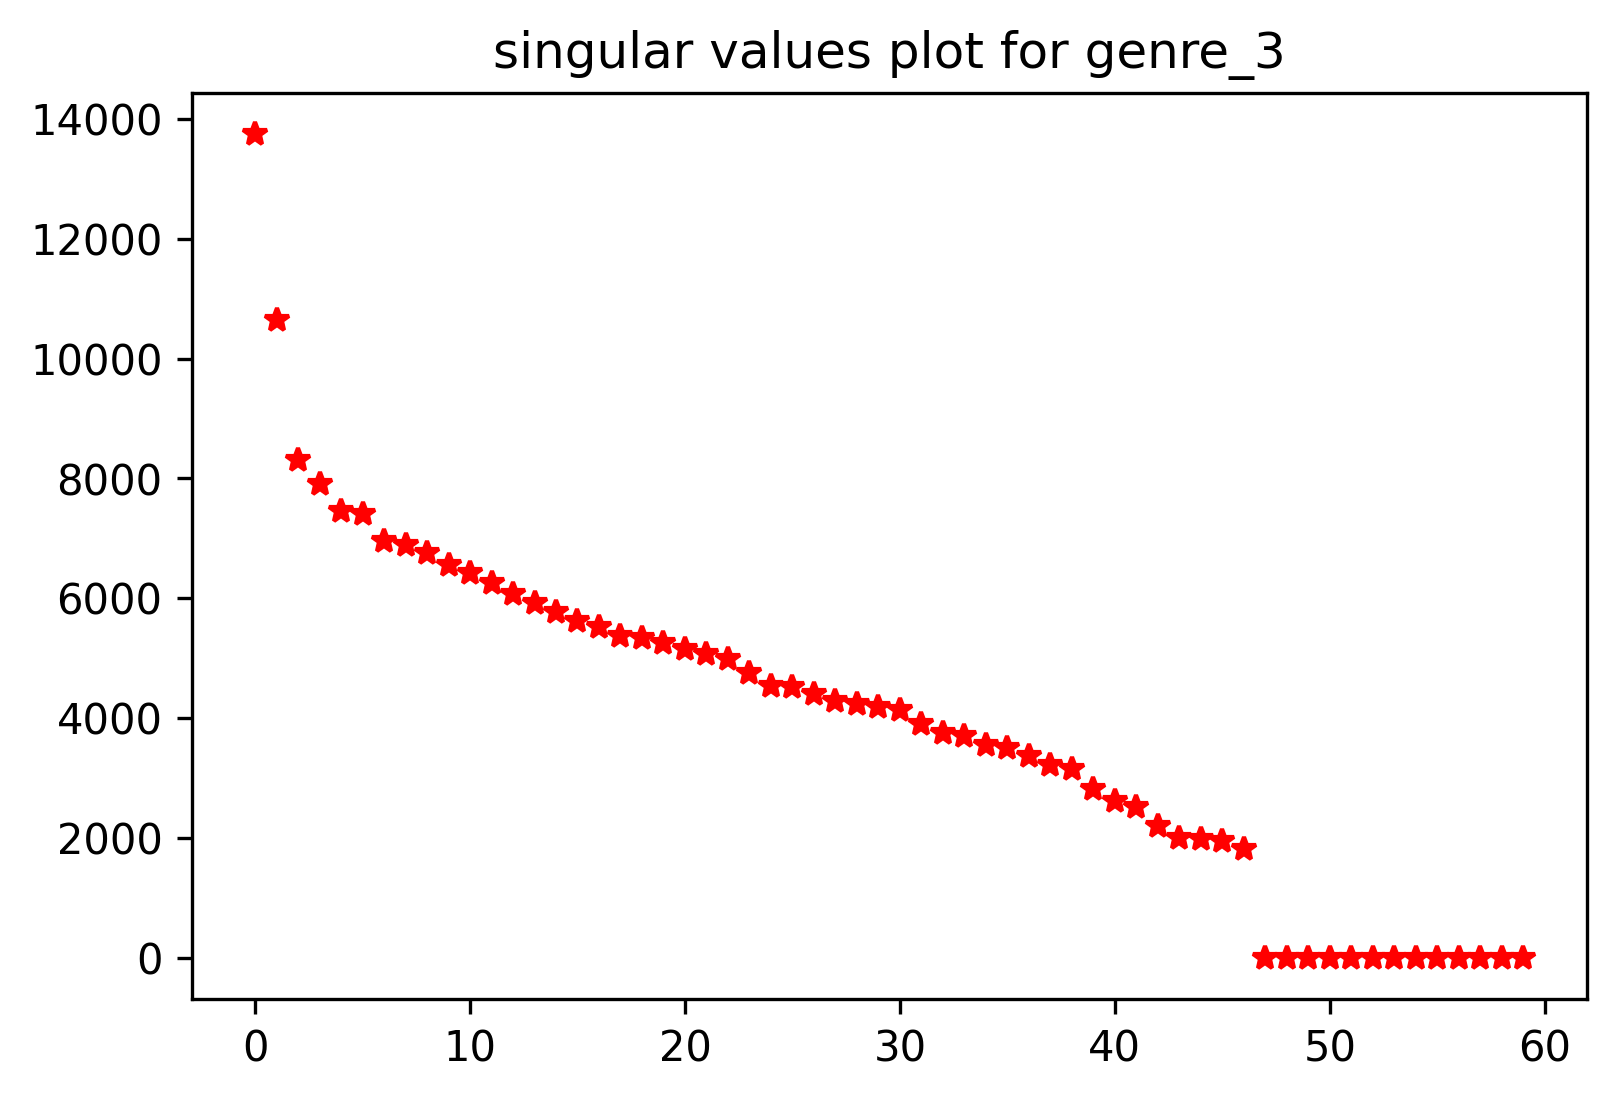
\includegraphics[width=4in]{image/s3_plot.png}
        \caption{Singular Value Plot for Genre 3}
        \label{fig:svd}
    \end{figure}
    \end{par}